%! Author = adnansiddiquei
%! Date = 19/03/2024

\section{Overview of Diffusion Model Implementation}\label{sec:q1a}
\subsection{coursework\_starter.ipynb}\label{subsec:q1a}
The code provided in the coursework\_starter.ipynb notebook trains a regular denoising diffusion probabilistic model
(DDPM) on the MNIST dataset, using the \inlinecode{pytorch} library.
This section provides a detailed explanation of how the given coursework\_starter.ipynb code works.
The notation used in this section adheres to the conventions used in Ch.18 of Understanding Deep Learning, Prince~\cite{prince}.

\subsubsection{The Data}\label{subsubsec:data}
The code loads the MNIST training dataset (60000 images) and preprocesses it with \inlinecode{transforms.toTensor} which converts
the image to a tensor and scales it to the range $[0, 1]$, followed by \inlinecode{transforms.Normalize((0.5,), (1.0))}
which shifts the range to $[-0.5, 0.5]$.
The scaling and range shift can help improve the training dynamics.
Given that MNIST images are grayscale (a single channel), the input dimensions are 1x28x28.
The dataset is then loaded into a \inlinecode{DataLoader} object with a batch size of 128, yielding 468 batches per
epoch.

\subsubsection{The CNN Model}\label{subsubsec:cnn-model}
The code defines a Convolutional Neural Network \inlinecode{CNN} class which is the neural network that is used to
learn the diffusion process - the noise that is added to the image at each step.
This is instantiated with 5 hidden layers, each outputting: 16, 32, 32, 16, 1 channels respectively, with a kernel size
of 7 at the first 4 layers, and a kernel size of 3 at the last layer.
Each of the first 4 hidden layers (defined in the \inlinecode{CNNBlock} class) are composed of a 2D convolutional layer
(with 0-padding on the edges) followed by a normalisation layer (\inlinecode{LayerNorm} which normalises each input to
standard normal) and a GELU activation function.
The normalisation stabilises the activations and places them in the transition range of the GELU function, which allows
for full use of the GELU's characteristics.

Decoder models for the diffusion process can either be a set of multiple models, each trained to revert the noise at
a particular step, or a single model trained to revert the noise at any given step by injecting information about the
time step into the model.
This CNN is the latter, and the \inlinecode{forward} function adds a time step dependent embedding to the pre-activations
of the second layer so that the CNN can learn to revert the noise at any given step.

\subsubsection{The DDPM Model}\label{subsubsec:ddpm-model}
\begin{figure}[t]
    \centering
    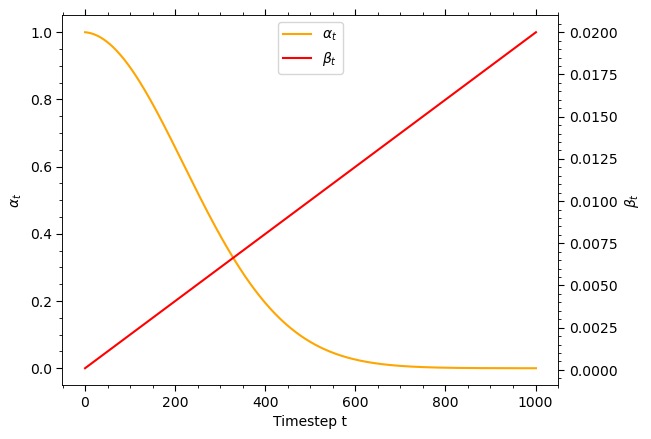
\includegraphics[width=0.8\textwidth]{figures/q1a_noise_schedule}
    \caption{A plot of $\beta_{t}$ and $\alpha_{t}$ for the linear noise schedule used in coursework\_starter.ipynb.
        This figure illustrates that MNIST images transition for noiseless to standard normally distributed noise
        over 1000 steps, with most of the noise being added by about the 600'th step.}
    \label{fig:q1a_noise_schedule}
\end{figure}

The training and sampling process is defined within the \inlinecode{DDPM} class, which contains a \inlinecode{forward}
function that defines the forward pass of the model and a
\inlinecode{sample} function that generates new MNIST data samples by iterating backwards through the diffusion process.
The DDPM is instantiated with the CNN defined above and a linear noise schedule with $\beta_{t}$ in the range $[10^{-4},
0.02]$ across 1000 steps, as shown in Figure~\eqref{fig:q1a_noise_schedule}, where $\beta_{t}$ and $\alpha_{t}$ are as
defined in Ch.18 Prince~\cite{prince}.

\begin{figure}[t]
    \centering
    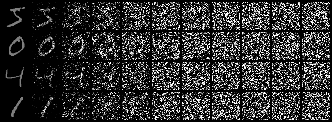
\includegraphics[width=0.8\textwidth]{figures/q1a_image_noising}
    \caption{An illustration of the linear noise schedule applied to the first 4 MNIST images in the training datastet.
        The first column shows the original 28x28 image, and the subsequent 10 columns show the image after 100 steps
        of the diffusion process.
        The final column shows the image after 1000 steps.}
    \label{fig:q1a_image_noising}
\end{figure}

The \inlinecode{forward} function samples 128 (the batch size) random $\alpha_{t}$ values from the noise schedule and
a standard normally distributed noise tensor of shape \inlinecode{(128, 1, 28, 28)}, and degrades every image in the batch
with the noise according to Equation~\eqref{eq:noise-schedule}~\cite{prince}.
\begin{equation}\label{eq:noise-schedule}
    z_{t} = \sqrt{\alpha_{t}} \cdot \mathbf{x} + \sqrt{1 - \alpha_{t}} \cdot \mathbf{\epsilon}
\end{equation}
Figure~\eqref{fig:q1a_image_noising} illustrates the diffusion process.
This batch of 128 noisy MNIST images (degraded to different extents) is then passed through the CNN (along with the
corresponding time steps) to make a prediction on the noise that was added to the image at the corresponding step.
The function returns the loss between the actual noise and this predicted noise as the mean squared error between the
two.

\begin{figure}[t]
    \centering
    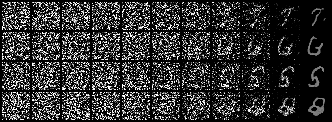
\includegraphics[width=0.8\textwidth]{figures/q1a_image_reconstruction}
    \caption{An illustration of the generation process.
        This is the generation of 4 new MNIST samples from the model trained with the default parameters in the
        coursework\_starter.ipynb notebook.
        The first column shows the randomly sampled noise, the next 10 columns illustrate the image after 100 steps of
        decoding, with the final column showing the final generated image.}
    \label{fig:q1a_image_reconstruction}
\end{figure}
The \inlinecode{sample} function can generate new MNIST samples by iterating backwards through the diffusion process
using the learned parameters of the CNN, and a random sample of standard normal noise.
Figure \eqref{fig:q1a_image_reconstruction} illustrates the generation process.

\subsubsection{The training loop}\label{subsubsec:training-loop}
The training loop iterates over 100 epochs, using the Adam optimiser and a learning rate of $2 \times 10^{-4}$,
saving generated samples from the model at every epoch along with the loss at each epoch.
